% Resultate
\section{Resultate}

\textsc{Kort} besteht aus fünf verschiedenen Hauptmasken.
Diese sind in der Applikation über die Tabs im unteren Bereich erreichbar.

\subsection{Maske: Aufträge}
In dieser Maske werden dem Benutzer alle noch nicht gelösten Fehler in seiner Umgebung als Markierungen auf der Karte angezeigt.
Die Fehleranzahl ist dabei auf die 25 nächstgelegenen Fehler limitiert.

Beim Klick auf einen Fehler wird der Benutzer gefragt, ob er diesen auch wirklich lösen kann.
Bestätigt er wird ihm der Fehler im Detail angezeigt.
In dieser Detailansicht wir ihm zudem je nach Fehlertyp ein Text- oder ein Auswahlfeld angezeigt in welchem er die Antwort eingeben bzw. auswählen kann. 

Zusätzlich hat er die Möglichkeit sich den Fehler nochmals auf der Karte anzuzeigen zu lassen.
Dabei wird dieser nicht nur als Markierung dargestellt sondern als ein Geometrie-Objekt entsprechend den OpenStreetMap-Daten.
Eine Strasse wird dabei beispielsweise als Linie dargestellt und ein Gelände als Polygon.

\begin{figure}[H]
\subfigure{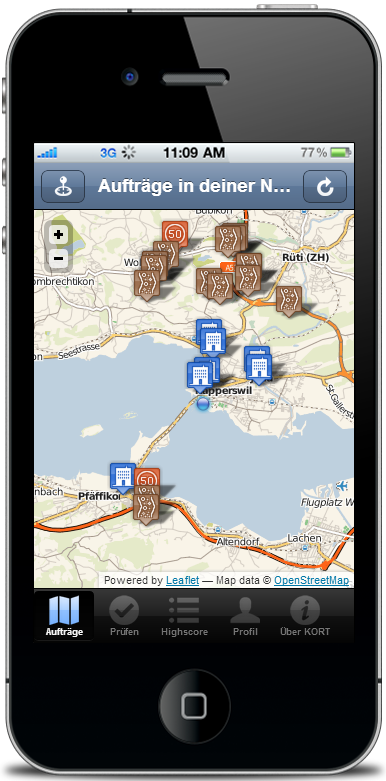
\includegraphics[width=0.3\textwidth]{images/screenshots/kort-screenshot-bugmap}}
\hfill
\subfigure{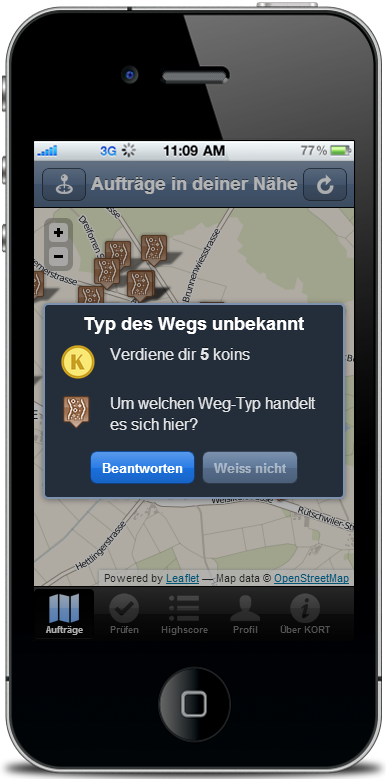
\includegraphics[width=0.3\textwidth]{images/screenshots/kort-screenshot-bugmap_message_box}}
\hfill
\subfigure{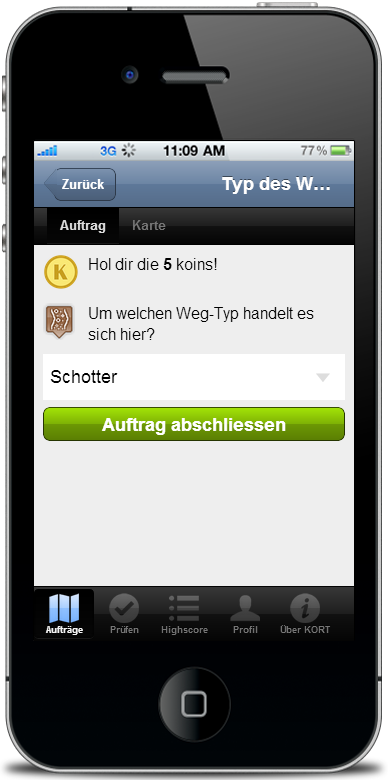
\includegraphics[width=0.3\textwidth]{images/screenshots/kort-screenshot-fix}}
\caption{Maske: Aufträge}
\end{figure}

\subsection{Maske: Prüfen}
In der Prüfen-Maske werden dem Benutzer die Lösungen angezeigt, welche noch zu überprüfen sind.
Diese sind dabei nach der Anzahl noch nötiger positiver Überprüfungen gruppiert.
So soll erreicht werden, dass Lösungen die schon bald an OpenStreetMap zurückgesendet werden können bevorzugt behandelt werden.
In der Liste werden maximal 25 Überprüfungen angezeigt.

Sobald er einen Eintrag anklickt, wird ihm der Fehler auf der Karte angezeigt inklusiver der eingetragenen Lösung.
Er kann nun beurteilen, ob ihm diese Lösung korrekt oder eher falsch erscheint.

\begin{figure}[H]
\subfigure{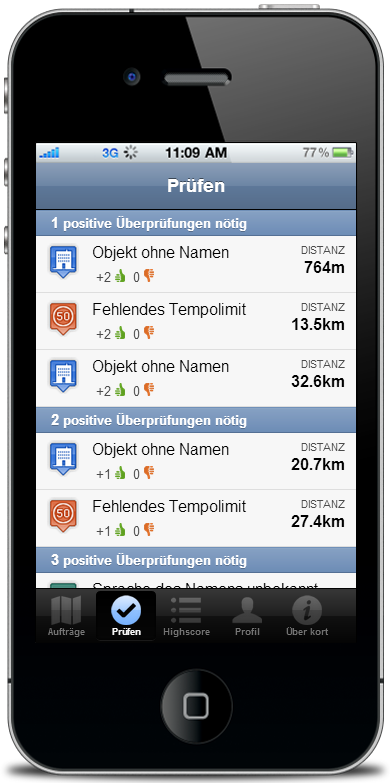
\includegraphics[width=0.3\textwidth]{images/screenshots/kort-screenshot-validation}}
\hfill
\subfigure{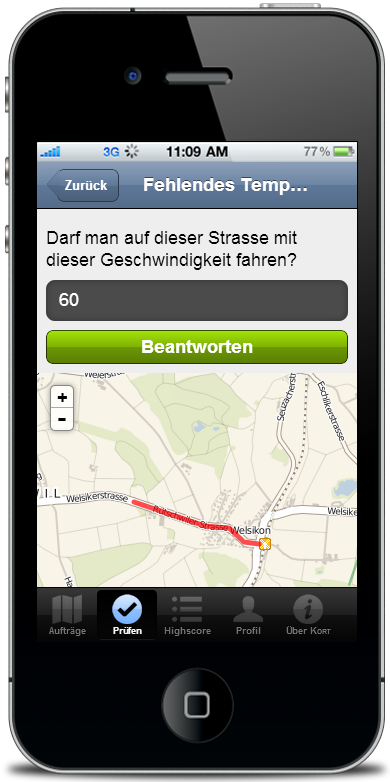
\includegraphics[width=0.3\textwidth]{images/screenshots/kort-screenshot-vote}}
\hfill
\subfigure{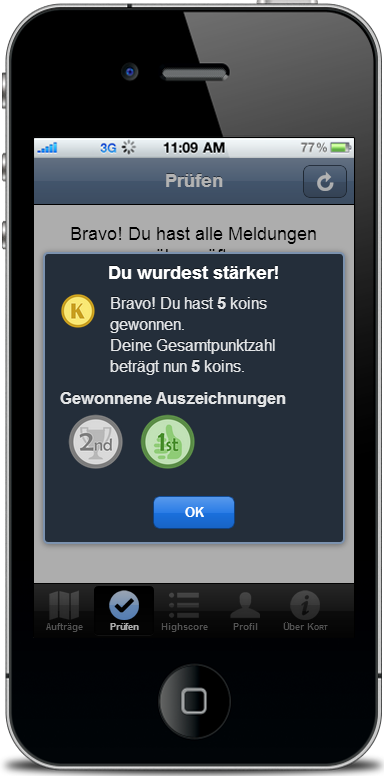
\includegraphics[width=0.3\textwidth]{images/screenshots/kort-screenshot-reward}}
\caption{Maske: Prüfen}
\end{figure}

\subsection{Maske: Highscore}
In der Highscore werden die Benutzer abhängig der Anzahl von ihnen gewonnener Punkte (sog. \emph{koins}) sortiert.
Es werden jeweils die ersten zehn Platzierungen angezeigt. Falls man selbst nicht zu diesen gehört wird zusätzlich eine Zeile mit seiner eigenen Platzierung angezeigt.

\subsection{Maske: Profil}
Im Profil findet man eine Zusammenfassung seiner persönlichen Spielaktivitäten.
Man sieht die Gesamtanzahl der gesammelten \emph{koins} und eine Übersicht der gewonnen Auszeichnungen

\subsection{Maske: Über Kort}
Auf der \emph{Über Kort}-Seite werden allgemeine Informationen zur Applikation angezeigt.

\begin{figure}[H]
\subfigure{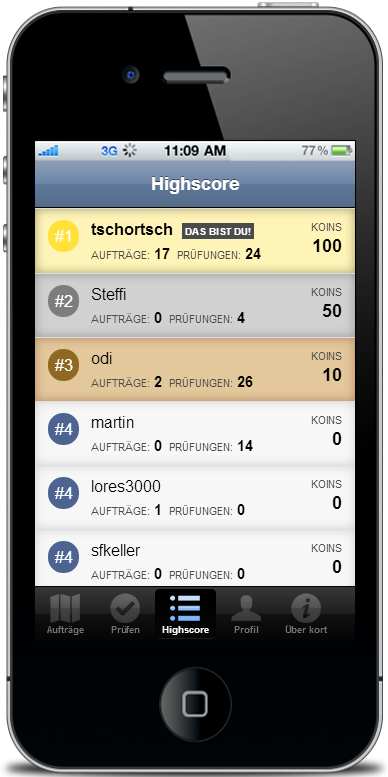
\includegraphics[width=0.3\textwidth]{images/screenshots/kort-screenshot-highscore}}
\hfill
\subfigure{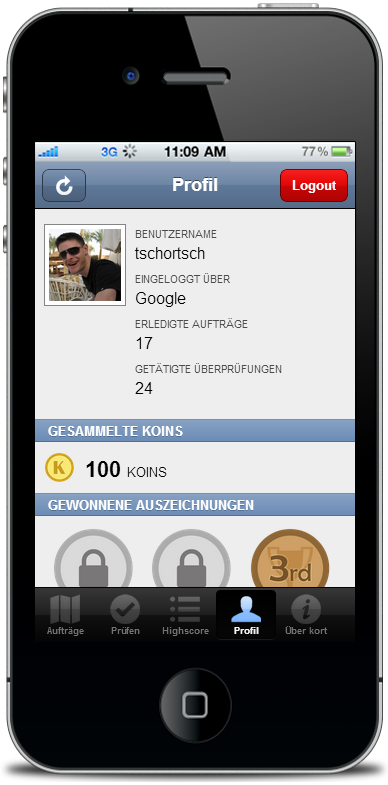
\includegraphics[width=0.3\textwidth]{images/screenshots/kort-screenshot-profile}}
\hfill
\subfigure{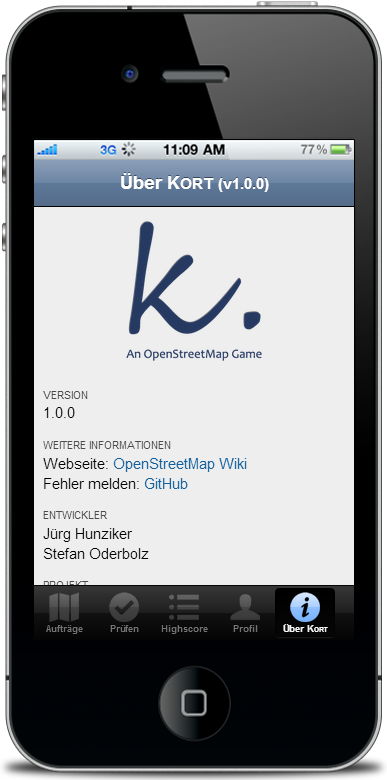
\includegraphics[width=0.3\textwidth]{images/screenshots/kort-screenshot-about}}
\caption{Masken: Highscore / Profil / Über Kort}
\end{figure}